\documentclass[UTF8]{xjuthesis}

\graphicspath{{figures/}}

%学位类型
\degreetype{硕士}

%中文题目
\cntitle{新疆大学硕士学位论文 \LaTeX \\ 模板使用指南(非官方)}
%英文题目
\entitle{Master thesis of Xinjiang university guide to using \LaTeX ~template \\ (unofficial)}

\author{某·某}                            % 研究生姓名
\subject{某某工程}                        % 学科
\researchinterest{某某某与某某某}          % 研究方向
\advisor{某某某}                             % 导师姓名
\advisortitle{教授}                        % 导师职称

\defenddate{20xx年xx月xx日}                % 论文答辩日期
\authorizedate{~~~~~~~~~年~~~~~月~~~~~日}             % 学位授予日期

\declarationdate{20xx年x月xx日}

\begin{document}


%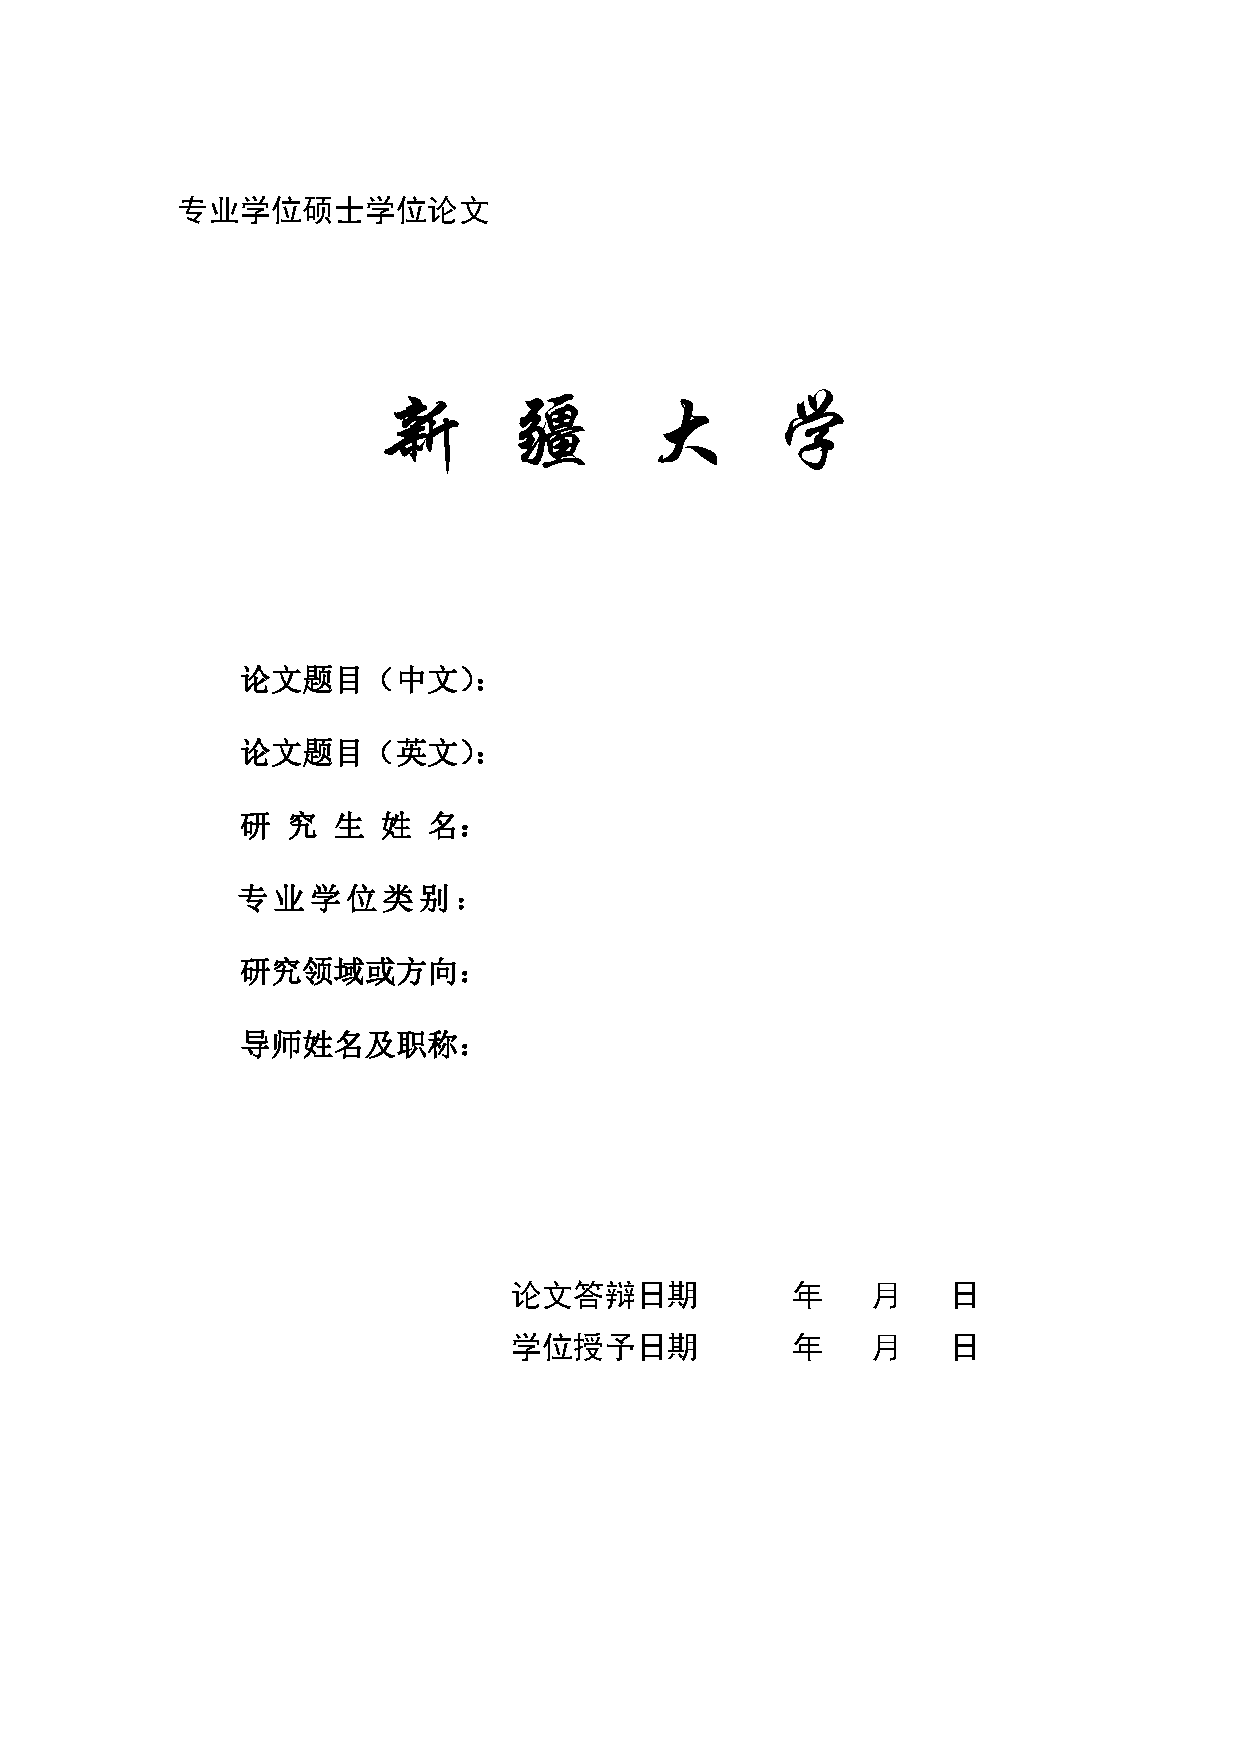
\includepdf[pages={1}]{1.pdf}

%封面
\maketitilepage

\frontmatter

%摘要
\begin{cnabstract}
	
	中文摘要部分的标题为“摘要”,“摘要”中间空1个汉字符,用黑体三号字,居中书写,单倍行距,段前空24磅,段后空18磅。
	
	摘要正文应说明本论文的研究目的、方法、成果和结论,要突出本论文的创造性成果或新见解,语言力求精炼、准确,摘要中不要出现图片、图表、表格或其他插图材料。中文摘要控制在800-1000汉字(符),且篇幅限制在1-2页内书写。摘要内容用宋体字小四号书写,两端对齐,行距为固定值20磅,段前、段后均为0行,首行缩进2字符。
	
	论文的关键词,是为了文献标引工作从论文中选取出来用以表示全文主题内容信息的单词或术语,关键词3-5个,另起一段用宋体字小四号书写,两端对齐,“关键词”三个字加粗。每个关键词之间用英文分号“;”间隔。
	
	
	\cnkeywords{摘要;中文}
	
\end{cnabstract}

\begin{enabstract}
	
	英文摘要部分的标题为“Abstract”,用Arial体三号字,加粗,居中书写,单倍行距,段前空24磅,段后空18磅。摘要内容用小四号Times New Roman字体书写,两端对齐,行距为固定值20磅,段前、段后均为0行,首行缩进2字符,标点符号用英文标点符号。“Key Words”与中文摘要部分的关键词对应,另起一段用小四号Times New Roman字体书写,两端对齐,“Key Words”两个单词加粗。每个关键词之间用英文分号“;”间隔。
	
	英文摘要部分的标题为“Abstract”,用Arial体三号字,加粗,居中书写,单倍行距,段前空24磅,段后空18磅。摘要内容用小四号Times New Roman字体书写,两端对齐,行距为固定值20磅,段前、段后均为0行,首行缩进2字符,标点符号用英文标点符号。“Key Words”与中文摘要部分的关键词对应,另起一段用小四号Times New Roman字体书写,两端对齐,“Key Words”两个单词加粗。每个关键词之间用英文分号“;”间隔。
	
	英文摘要部分的标题为“Abstract”,用Arial体三号字,加粗,居中书写,单倍行距,段前空24磅,段后空18磅。摘要内容用小四号Times New Roman字体书写,两端对齐,行距为固定值20磅,段前、段后均为0行,首行缩进2字符,标点符号用英文标点符号。“Key Words”与中文摘要部分的关键词对应,另起一段用小四号Times New Roman字体书写,两端对齐,“Key Words”两个单词加粗。每个关键词之间用英文分号“;”间隔。
	
	英文摘要部分的标题为“Abstract”,用Arial体三号字,加粗,居中书写,单倍行距,段前空24磅,段后空18磅。摘要内容用小四号Times New Roman字体书写,两端对齐,行距为固定值20磅,段前、段后均为0行,首行缩进2字符,标点符号用英文标点符号。“Key Words”与中文摘要部分的关键词对应,另起一段用小四号Times New Roman字体书写,两端对齐,“Key Words”两个单词加粗。每个关键词之间用英文分号“;”间隔。
	
	英文摘要部分的标题为“Abstract”,用Arial体三号字,加粗,居中书写,单倍行距,段前空24磅,段后空18磅。摘要内容用小四号Times New Roman字体书写,两端对齐,行距为固定值20磅,段前、段后均为0行,首行缩进2字符,标点符号用英文标点符号。“Key Words”与中文摘要部分的关键词对应,另起一段用小四号Times New Roman字体书写,两端对齐,“Key Words”两个单词加粗。每个关键词之间用英文分号“;”间隔。
	
	英文摘要部分的标题为“Abstract”,用Arial体三号字,加粗,居中书写,单倍行距,段前空24磅,段后空18磅。摘要内容用小四号Times New Roman字体书写,两端对齐,行距为固定值20磅,段前、段后均为0行,首行缩进2字符,标点符号用英文标点符号。“Key Words”与中文摘要部分的关键词对应,另起一段用小四号Times New Roman字体书写,两端对齐,“Key Words”两个单词加粗。每个关键词之间用英文分号“;”间隔。
	
	英文摘要部分的标题为“Abstract”,用Arial体三号字,加粗,居中书写,单倍行距,段前空24磅,段后空18磅。摘要内容用小四号Times New Roman字体书写,两端对齐,行距为固定值20磅,段前、段后均为0行,首行缩进2字符,标点符号用英文标点符号。“Key Words”与中文摘要部分的关键词对应,另起一段用小四号Times New Roman字体书写,两端对齐,“Key Words”两个单词加粗。每个关键词之间用英文分号“;”间隔。
	
	论文摘要的中文版与英文版文字内容要对应,都采用双面打印。
	
	
	\enkeywords{Abstract; english}
	
\end{enabstract}

%目录
\tableofcontents

% 符号对照表
\begin{denotation}
	\begin{center}
		\xiaosi
		\begin{tabularx}{\textwidth}{l@{\hspace{2cm}}@{\extracolsep{2cm}}l}
			$ \alpha $ & Alpha \\
			$ \beta $ & Beta \\
			$ \gamma $ & Gamma \\
			$ \Delta $ & Delta \\
			$ \theta $ & Theta \\
			$ \lambda $ & Lambda \\
			$ \pi $ & Pi \\
			$ \Sigma $ & Sigma \\
			$ \omega $ & Omega \\
		\end{tabularx}
	\end{center}
\end{denotation}



\mainmatter

%正文
\chapter{第一章 Aa 1}

章序号采用阿拉伯数字,章序号与标题名之间空一个汉字符。采用黑体三号字,居中书写,单倍行距,段前空24磅,段后空18磅。论文的摘要、目录、主要符号对照表、参考文献、附录、致谢、学位论文独创性声明及学位论文知识产权权属声明、个人简历、在学期间发表的学术论文与研究成果等部分的标题与章标题属于同一等级,也使用上述格式;英文摘要部分的标题“Abstract”采用Arial体三号字加粗。

在写作指南中并没有给出章节目录英文字体格式,本模板按下面的组合定义格式:

\begin{enumerate}
	\item 宋体 + Times New Roman
	\item 黑体 + Arial
	\item 公式字体选择为:Latin Modern Math
	\item 编程字体选择为:黑体 + Courier New
\end{enumerate}

\section{一级节标题 Aa 1}

一级节标题,例如:“2.1  实验装置与实验方法”。
节标题序号与标题名之间空一个汉字符(下同)。采用黑体四号(14pt)字居左书写,行距为固定值20磅,段前空24磅,段后空6磅。


\subsection{二级节标题}

二级节标题,例如:“2.1.1  实验装置”。
采用黑体13pt字居左书写,行距为固定值20磅,段前空12磅,段后空6磅。


\subsubsection{三级节标题}

三级节标题,例如:“2.1.2.1  归纳法”。
采用黑体小四号(12pt)字居左书写,行距为固定值20磅,段前空12磅,段后空6磅。一般情况下不建议使用三级节标题。


\section{论文段落的文字部分(正文)}

采用小四号(12pt)字,汉字用宋体,英文用Times New Roman体,两端对齐书写,首行缩进2个字符。行距为固定值20磅(段落中有数学表达式时,可根据表达需要设置该段的行距),段前空0磅,段后空0磅。
论文的附录、致谢、学位论文独创性声明及学位论文知识产权权属声明部分部分中的正文也使用上述格式。

\subsection{脚注}

正文中某句话需要具体注释、且注释内容与正文内容关系不大时可以采用脚注方式。在正文中需要注释的句子结尾处用“圆圈数字”样式的数字编排序号,以“上标”字体标示在需要注释的句子末尾。在当页下部书写脚注内容。
脚注内容采用宋体小五号字,按两端对齐格式书写,单倍行距,段前段后均为0。脚注的序号按页编排,不同页的脚注要重新编号。详细规定见本页脚注。 

在这里设置了,一页脚注个数不能超过9个。

脚注测试~\footnote{每页脚注从1开始,下一页编号清零,重新计数。},见页脚\footnote{每页脚注从1开始,下一页编号清零,重新计数。每页脚注从1开始,下一页编号清零,重新计数。每页脚注从1开始,下一页编号清零,重新计数。每页脚注从1开始,下一页编号清零,重新计数。}。

\subsection{参考文献}

新疆大学研究生学位论文中的参考文献采用GB/T 7714—2015推荐的顺序编码制格式著录。参考文献(即引文出处)的类型以单字母方式标识。

“参考文献”四个字的格式与章标题的格式相同。参考文献表的正文部分用五号字,汉字用宋体,英文用Times New Roman体,两端对齐,行距采用固定值16磅,段前空3磅,段后空0磅,缩进左右侧均为0。
参考文献的内容要尽量写在同一页内。遇有被迫分页的情况,可通过“留白”或微调本页行距的方式尽量将同一条文献内容放在一页。
关于参考文献的著录格式以及在正文中的标注方法详细见第3章。

参考文献引用测试~\cite{born1981}。

参考文献引用测试~\cite{knuth1984}。

多个参考文献引用测试~\cite{born1981,knuth1984}。


\subsection{超链接}

\url{https://cn.bing.com/}
\chapter{第二章}

\section{图}

图要精选,要具有自明性,切忌与表及文字表述重复。

图要清楚,但坐标比例不要过分放大,同一图上不同曲线的点要分别用不同形状的标识符标出。

图中的术语、符号、单位等应与正文表述中所用一致。

图序与图名,例如:“图2.1  发展中国家经济增长速度的比较(1960-2000)”。

图2.1是图序,是“第2章第1个图”的序号,其余类推。图序与图名置于图的下方,采用宋体11pt字居中书写,段前空6磅,段后空12磅,行距为单倍行距,图序与图名文字之间空一个汉字符宽度。

图中标注的文字采用9~10.5pt,以能够清晰阅读为标准。专用名字代号、单位可采用外文表示,坐标轴题名、词组、描述性的词语均须采用国家通用语言文字。

如果一个图由两个或两个以上分图组成时,各分图分别以(a)、(b)、(c)……作为图序,并须有分图名。



\subsection{图片插入演示}

\begin{figure}[hbt]
	\centering
	
\includegraphics[width=0.5\textwidth]{xju_logo}
	\caption{图片名称}
	\label{xju_logo}
\end{figure}

图片引用演示:图\ref{xju_logo}。

\subsubsection{多图插入演示}


\begin{figure}[!htb]
	\centering
	\begin{subfigure}[t]{0.24\linewidth}
		\captionsetup{justification=centering} %子图caption居中
		\begin{minipage}[b]{1\linewidth}
			
\includegraphics[width=1\linewidth]{xju_logo}
			\caption{第一个子图}
			\label{xju_logo1:subfig1}
		\end{minipage}
	\end{subfigure}
	\begin{subfigure}[t]{0.24\linewidth}
		\captionsetup{justification=centering} %子图caption居中
		\begin{minipage}[b]{1\linewidth}
			
\includegraphics[width=1\linewidth]{xju_logo}
			\caption{第二个子图}
			\label{xju_logo1:subfig2}
		\end{minipage}
	\end{subfigure}
	\caption{并排排布局示例。(a)表示什么什么什么么什么什么什么什么什什么什么什么什么什么什么么什么什么什么什么什么什么什么什么。(b)表示什么什么什么什么什么什么什么什么什么什么什么什么什么什么什么什么。}
	\label{xju_logo1}
\end{figure}

多图子图引用演示:图\ref{xju_logo1:subfig1}。

\begin{figure}[!htb]
	\centering
	\begin{subfigure}[t]{0.15\linewidth}
		\captionsetup{justification=centering}
		\begin{minipage}[b]{1\linewidth}
			
\includegraphics[width=1\linewidth]{xju_logo}
			\caption{}
		\end{minipage}
	\end{subfigure}\\
	\begin{subfigure}[t]{0.15\linewidth}
		\captionsetup{justification=centering}
		\begin{minipage}[b]{1\linewidth}
			
\includegraphics[width=1\linewidth]{xju_logo}
			\caption{}
		\end{minipage}
	\end{subfigure}
	\caption{竖排布局示例}
	\label{xju_logo2}
\end{figure}


\begin{figure}[!htb]
	\centering
	\begin{subfigure}[t]{0.13\linewidth}
		\captionsetup{justification=centering}
		\begin{minipage}[b]{1\linewidth}
			
\includegraphics[width=1\linewidth]{xju_logo} \vspace{-1ex} \vfill
			
\includegraphics[width=1\linewidth]{xju_logo}
			\caption{}
		\end{minipage}
	\end{subfigure}
	\begin{subfigure}[t]{0.13\linewidth}
		\captionsetup{justification=centering}
		\begin{minipage}[b]{1\linewidth}
			
\includegraphics[width=1\linewidth]{xju_logo} \vspace{-1ex} \vfill
			
\includegraphics[width=1\linewidth]{xju_logo}
			\caption{}
		\end{minipage}
	\end{subfigure}
	\caption{竖排多图横排布局}
	\label{xju_logo3}
\end{figure}

\begin{figure}[!htb]
	\centering
	\begin{subfigure}[t]{0.3\linewidth}
		\captionsetup{justification=centering}
		\begin{minipage}[b]{1\linewidth}
			
\includegraphics[width=0.45\linewidth]{xju_logo}
			
\includegraphics[width=0.45\linewidth]{xju_logo}
			\caption{}
		\end{minipage}
	\end{subfigure}\\
	\begin{subfigure}[t]{0.3\linewidth}
		\captionsetup{justification=centering}
		\begin{minipage}[b]{1\linewidth}
			
\includegraphics[width=0.45\linewidth]{xju_logo}
			
\includegraphics[width=0.45\linewidth]{xju_logo}
			\caption{}
		\end{minipage}
	\end{subfigure}
	\caption{横排多图竖排布局}
	\label{xju_logo4}
\end{figure}
	
\section{表}
	
\begin{table}[htb]
	\centering
	\caption{表格为三线表}
	\label{table1}
	\begin{tabular}{llllll}
		\toprule[1.5pt]
		& A & \emph{B} & \textit{C} & D & E \\
		\midrule[1pt]
		1 & 000 & 111 & Aa & - & 表格	\\
		2 & 000 & 111 & Aa & - & 表格	\\
		3 & 000 & 111 & Aa & - & 表格	\\
		\bottomrule[1.5pt]
	\end{tabular}
\end{table}

表格引用演示:表\ref{table1}。

\begin{table}[htb]
	\noindent\begin{minipage}{0.5\textwidth}
		\centering
		\caption{第一个并排子表格}
		\label{table2:subtab1}
		\begin{tabular}{p{2cm}p{2cm}}
			\toprule[1.5pt]
			aaa & bbb \\
			\midrule[1pt]
			111 & 111 \\
			111 & 111 \\
			111 & 111 \\
			\bottomrule[1.5pt]
		\end{tabular}
	\end{minipage}
	\begin{minipage}{0.5\textwidth}
		\centering
		\caption{第二个并排子表格}
		\label{table2:subtab2}
		\begin{tabular}{p{2cm}p{2cm}}
			\toprule[1.5pt]
			ccc & ddd \\
			\midrule[1pt]
			222 & 222 \\
			222 & 222 \\
			222 & 222 \\
			\bottomrule[1.5pt]
		\end{tabular}
	\end{minipage}
\end{table}

子表格引用演示:表\ref{table2:subtab1}。

\begin{table}[htb]
	\centering
	\begin{minipage}[t]{6cm} % 如果想在表格中使用脚注,minipage是个不错的办法
		\caption{表格脚注演示:表格名表格名表格名表格名表格名表格名}
		\label{table3}
		\begin{tabular*}{\linewidth}{lp{6cm}}
			\toprule[1.5pt]
			{\heiti 内容} & {\heiti 内容} \\
			\midrule[1pt]
			aaa & 内容内容内容\footnote{表格中的脚注}\\
			bbb & 内容内容内容\\
			ccc & 内容内容内容\\
			ddd\footnote{再来一个} & 内容\\
			\bottomrule[1.5pt]
		\end{tabular*}
	\end{minipage}
\end{table}


\begin{table}[htb]
	\centering
	\caption{表格}
	\label{table4}
	\begin{minipage}[c]{0.8\linewidth}
		\begin{tabular*}{\linewidth}{lp{10cm}}
			\toprule[1.5pt]
			内容 & 内容 \\
			\midrule[1pt]
			aaa$^{*}$ & 内容内容内容内容内容内容内容内容内容内容内容内容内容\\
			bbb & 内容内容内容内容内容内容内容内容内容内容\\
			ccc & 内容内容内容内容内容内容内容内容内容内容内容内容内容内容\\
			ddd & 内容内容内容内容内容内容内$^{**}$容内容内容内容\\
			\bottomrule[1.5pt]
		\end{tabular*}\\[2pt]
		注:数据来源。\\
		*:a部\\
		**:b部
	\end{minipage}
\end{table}


\subsection{跨页表格}

\begin{longtable}[h]{c*{8}{c}}
	\caption{数据}
	\label{table2}\\
	\toprule[1.5pt]
	表格 & \multicolumn{1}{c}{列1} & \multicolumn{1}{c}{列2} & \multicolumn{1}{c}{列3} & \multicolumn{1}{c}{列4}
	& \multicolumn{1}{c}{列5} & \multicolumn{1}{c}{列6} & \multicolumn{1}{c}{列7} & \multicolumn{1}{c}{列8} \\
	& \multicolumn{1}{c}{a} & \multicolumn{1}{c}{b} &
	\multicolumn{1}{c}{c} & \multicolumn{1}{c}{d} & \multicolumn{1}{c}{e} &  \multicolumn{1}{c}{f} & \multicolumn{1}{c}{g} & \multicolumn{1}{c}{h} \\
	\midrule[1pt]
	% 第一页表头内容
	\endfirsthead
		\multicolumn{9}{c}{续表~\thetable\hskip1em 数据} \\
	\hline
	% 跨页表头内容
	\endhead
	\hline
	% 跨页表尾内容
	\endfoot
	% 最后一页表尾内容
	\endlastfoot
	A & 0.00 & 0.000 & 0.000 & 0.000 & 0.000 & 0.000 & 0.000 & 0.000 \\
	B & 0.00 & 0.000 & 0.000 & 0.000 & 0.000 & 0.000 & 0.000 & 0.000 \\
	C & 0.00 & 0.000 & 0.000 & 0.000 & 0.000 & 0.000 & 0.000 & 0.000 \\
	D & 0.00 & 0.000 & 0.000 & 0.000 & 0.000 & 0.000 & 0.000 & 0.000 \\
	E & 0.00 & 0.000 & 0.000 & 0.000 & 0.000 & 0.000 & 0.000 & 0.000 \\
	F & 0.00 & 0.000 & 0.000 & 0.000 & 0.000 & 0.000 & 0.000 & 0.000 \\
	G & 0.00 & 0.000 & 0.000 & 0.000 & 0.000 & 0.000 & 0.000 & 0.000 \\
	H & 0.00 & 0.000 & 0.000 & 0.000 & 0.000 & 0.000 & 0.000 & 0.000 \\
	I & 0.00 & 0.000 & 0.000 & 0.000 & 0.000 & 0.000 & 0.000 & 0.000 \\
	J & 0.00 & 0.000 & 0.000 & 0.000 & 0.000 & 0.000 & 0.000 & 0.000 \\
	K & 0.00 & 0.000 & 0.000 & 0.000 & 0.000 & 0.000 & 0.000 & 0.000 \\
	L & 0.00 & 0.000 & 0.000 & 0.000 & 0.000 & 0.000 & 0.000 & 0.000 \\
	M & 0.00 & 0.000 & 0.000 & 0.000 & 0.000 & 0.000 & 0.000 & 0.000 \\
	N & 0.00 & 0.000 & 0.000 & 0.000 & 0.000 & 0.000 & 0.000 & 0.000 \\
	O & 0.00 & 0.000 & 0.000 & 0.000 & 0.000 & 0.000 & 0.000 & 0.000 \\
	P & 0.00 & 0.000 & 0.000 & 0.000 & 0.000 & 0.000 & 0.000 & 0.000 \\
	Q & 0.00 & 0.000 & 0.000 & 0.000 & 0.000 & 0.000 & 0.000 & 0.000 \\
	R & 0.00 & 0.000 & 0.000 & 0.000 & 0.000 & 0.000 & 0.000 & 0.000 \\
	S & 0.00 & 0.000 & 0.000 & 0.000 & 0.000 & 0.000 & 0.000 & 0.000 \\
	T & 0.00 & 0.000 & 0.000 & 0.000 & 0.000 & 0.000 & 0.000 & 0.000 \\
	U & 0.00 & 0.000 & 0.000 & 0.000 & 0.000 & 0.000 & 0.000 & 0.000 \\
	\bottomrule[1.5pt]
\end{longtable}


\section{表达式}

表达式主要是指数字表达式,例如数学表达式,也包括文字表达式。

表达式采用与正文相同的字号居中书写,或另起一段空两个汉字符书写,一旦采用了上述两种格式中的一种,全文都要使用同一种格式。表达式应有序号,序号用括号括起来置于表达式右边行末,序号与表达式之间不加任何连线。

表达式行的行距为单倍行距,段前空6磅,段后空6磅。当表达式不是独立成行书写时,有表达式的段落的行距为单倍行距,段前空3磅,段后空3磅。

文中的表、图、表达式一律采用阿拉伯数字分章编号,例如:“表3.2”,“图2.5”,式“(3-1)”等。表达式在文字叙述中采用“式(3-1)”形式,在编号中用“(3-1)”形式。若图或表中有附注,采用英文小写字母顺序编号,附注写在图或表的下方。

\subsection{数学公式}

公式引用演示:公式\ref{equation1}。

\begin{equation}
	\label{equation1}
	y=kx+b
\end{equation}

\hspace{\ccwd} $x$ $\textemdash$ 解释什么什么;

\hspace{\ccwd} $k$ $\textemdash$ 解释什么什么;

\hspace{\ccwd} $b$ $\textemdash$ 解释什么什么;

\hspace{\ccwd} $y$ $\textemdash$ 解释什么什么;

\begin{align}
	y &= \sqrt{\frac{2}{\pi}} \int_{0}^{x} e^{-t^2}\cos(t) \, dt \\
	F &= X + Y
\end{align}

\begin{equation}
	\left\{\begin{array}{l}
		\nabla f({\mbox{\boldmath $x$}}^*)-\sum\limits_{j=1}^p\lambda_j\nabla g_j({\mbox{\boldmath $x$}}^*)=0\\[0.3cm]
		\lambda_jg_j({\mbox{\boldmath $x$}}^*)=0,\quad j=1,2,\cdots,p\\[0.2cm]
		\lambda_j\ge 0,\quad j=1,2,\cdots,p.
	\end{array}\right.
\end{equation}

\begin{equation}
	\begin{aligned}
		\int_{−\infty}^{\infty}f(x)dx & = \frac{1}{2\lambda}\int_{−\infty}^{\infty}e^{−\frac{|x−\mu|}{\lambda}}dx \\
		& = \frac{1}{2}\int_{−\infty}^{\infty}e^{−|t|}dt \\
		& = 1
	\end{aligned}
\end{equation}

\[
A = \begin{bmatrix}
	a & b \\
	c & d
\end{bmatrix},
B = \begin{bmatrix}
	e & f \\
	g & h
\end{bmatrix},
C = \begin{bmatrix}
	i & j \\
	k & l
\end{bmatrix},
D = \begin{bmatrix}
	m & n \\
	o & p
\end{bmatrix},
E = \begin{bmatrix}
	q & r \\
	s & t
\end{bmatrix}
\]


\subsection{数学相关}

从这里开始,学校就没有严格的格式要求,已发表的硕士论文也没有一个统一的格式,下面是本模板给出的方案,请使用者自行判断。

引用:定理\ref{theorem1}。

\begin{theorem}[\cite{born1981}]
	\label{theorem1}
	
	%	\setlength{\baselineskip}{20pt}         % 基准行间距
	%	\renewcommand{\baselinestretch}{1.0}   % 几倍行间距
	开始定理。。。
\end{theorem}

\begin{lemma}
	\label{lemma1}
	%\setlength{\baselineskip}{20pt}         % 基准行间距
	%\renewcommand{\baselinestretch}{1.0}   % 几倍行间距
	开始引理。。。
\end{lemma}

\begin{proposition}
	\label{proposition1}
	%\setlength{\baselineskip}{20pt}         % 基准行间距
	%\renewcommand{\baselinestretch}{1.0}   % 几倍行间距
	开始命题。。。
\end{proposition}

\begin{corollary}
	\label{corollary1}
	%\setlength{\baselineskip}{20pt}         % 基准行间距
	%\renewcommand{\baselinestretch}{1.0}   % 几倍行间距
	开始推论。。。
\end{corollary}

\begin{example}
	\label{example1}
	%\setlength{\baselineskip}{20pt}         % 基准行间距
	%\renewcommand{\baselinestretch}{1.0}   % 几倍行间距
	开始举例。。。
\end{example}

\begin{definition}
	\label{definition1}
	%\setlength{\baselineskip}{20pt}         % 基准行间距
	%\renewcommand{\baselinestretch}{1.0}   % 几倍行间距
	开始定义。。。
\end{definition}

\begin{remark}
	\label{remark1}
	%\setlength{\baselineskip}{20pt}         % 基准行间距
	%\renewcommand{\baselinestretch}{1.0}   % 几倍行间距
	开始。。。
\end{remark}

\begin{solution}
	\label{solution1}
	%\setlength{\baselineskip}{20pt}         % 基准行间距
	%\renewcommand{\baselinestretch}{1.0}   % 几倍行间距
	开始。。。
	$\hfill\blacksquare$ %% 以方块结尾
\end{solution}

\begin{proof*} %% 证明不编号
	%	\setlength{\baselineskip}{20pt}         % 基准行间距
	%	\renewcommand{\baselinestretch}{1.0}   % 几倍行间距
	开始证明。。。
	\begin{equation}
		A = \begin{bmatrix}
			1 & 1 & 1 \\
			1 & 1 & 1 \\
			2 & 1 & 1
		\end{bmatrix}
	\end{equation}
	
	$\hfill\blacksquare$ %% 以黑方块结尾
\end{proof*}


\subsection{编程相关}

\begin{algorithm}
	\caption{算法示例}
	\label{alg1}
	\begin{algorithmic}[1]
		\REQUIRE 相关输入。。。。
		
		\ENSURE 相关输出。。。
		
		\STATE 算法描述  % 只占用一个行号
		\FOR{$i \gets 1\cdots N$}
		\STATE 算法描述
		\FOR{\textbf{each} $j \gets 1\cdots K$}
		\STATE 算法描述
		\ENDFOR
		\ENDFOR
		\REPEAT
		\REPEAT
		\STATE 令$\tau\gets\tau+1$
		\UNTIL 内循环迭代终止条件
		\STATE 。。。
		\UNTIL 外循环迭代终止条件
	\end{algorithmic}
\end{algorithm}

\begin{center}
	\fbox{\parbox[t]{\textwidth}{
					aaa\\
					bbb\\
					ccc}}
\end{center}

以下代码为啥啥啥。。。

\begin{lstlisting}[language=C++]
#include <iostream>
#include <string>

class Person {
	public:
	// 构造函数Aa
	Person(std::string name, int age, std::string gender) {
		this->name = name;
		this->age = age;
		this->gender = gender;
	}
	
	// 成员函数 Aa
	void introduce() {
		std::cout << "My name is " << name << ", I'm " << age << " years old, and I'm a " << gender << "." << std::endl;
	}
	
	private:
	std::string name;
	int age;
	std::string gender;
};

int main() {
	// 创建一个 Person 对象
	Person p("Tom", 25, "male");
	
	// 调用成员函数
	p.introduce();
	
	return 0;
}

\end{lstlisting}


\begin{lstlisting}[language=python]
from datetime import datetime   
from playsound import playsound
alarm_time = input("Enter the time of alarm to be set:HH:MM:SS\n")
alarm_hour=alarm_time[0:2]
alarm_minute=alarm_time[3:5]
alarm_seconds=alarm_time[6:8]
alarm_period = alarm_time[9:11].upper()
print("Setting up alarm..")
while True:
	now = datetime.now()
	current_hour = now.strftime("%I")
	current_minute = now.strftime("%M")
	current_seconds = now.strftime("%S")
	current_period = now.strftime("%p")
		if(alarm_period==current_period):
			if(alarm_hour==current_hour):
				if(alarm_minute==current_minute):
					if(alarm_seconds==current_seconds):
					print("Wake Up!")
					playsound('audio.mp3') ## download the alarm sound from link
					break

\end{lstlisting}


\chapter{第三章}

\section{一级节标题}

内容。。。

\subsection{二级节标题}

内容。。。

\section{一级节标题}

内容。。。

\subsection{二级节标题}

内容。。。

\section{一级节标题}

内容。。。

\subsection{二级节标题}

内容。。。
\chapter{第四章}

\section{一级节标题}

内容。。。

\subsection{二级节标题}

内容。。。

\section{一级节标题}

内容。。。

\subsection{二级节标题}

内容。。。

\section{一级节标题}

内容。。。

\subsection{二级节标题}

内容。。。
\chapter{结论与展望}

\section{一级节标题}
 
内容。。。

\section{一级节标题}

内容。。。



%参考文献
\phantomsection
\addcontentsline{toc}{chapter}{参考文献}
\bibliography{ref/ref.bib}

%附录

\appendix
\backmatter
\chapter{附录名称}

\section{附录要求}

附录是与论文内容密切相关、但编入正文又影响整篇论文编排的条理和逻辑性的一些资料,例如某些重要的数据表格、数学推导、计算程序、统计表、计算机打印输出件等,是论文主体的补充内容,可根据需要设置。

附录的格式与正文相同,并依顺序用大写字母A,B,C,……编序号,如附录A,附录B,附录C,……。只有一个附录时也要编序号,即附录A。每个附录应有标题。附录序号与附录标题之间空一个汉字符。例如:“附录A  2011年新疆设施农业天敌昆虫统计数据”。

附录中的图、表、数学表达式、参考文献等另行编序号,与正文分开,一律用阿拉伯数字编码,但在数码前冠以附录的序号,例如“图A.1”,“表B.2”,“式(C-3)”等。


\chapter{附录2}

\section{附录内容}

公式

\begin{equation}
	y=kx+b
\end{equation}

\begin{theorem}
	定理
\end{theorem}

表格

\begin{table}[htb]
	\centering
	\caption{表格}
	\begin{tabular}{llllll}
		\toprule[1.5pt]
		& A & B & C & D & E \\
		\midrule[1pt]
		1 & 000 & 111 & Aa & - & 表格	\\
		2 & 000 & 111 & Aa & - & 表格	\\
		3 & 000 & 111 & Aa & - & 表格	\\
		\bottomrule[1.5pt]
	\end{tabular}
\end{table}

图

\begin{figure}[hbt]
	\centering
	
\includegraphics[width=0.4\textwidth]{xju_logo}
	\caption{图片名称}
\end{figure}


%致谢
\begin{acknowledgement}
	致谢:用于评审、答辩、审议学位及提交学校存档的论文,致谢对象一般是对完成学位论文在学术上有较重要帮助的团体和人士。
	致谢限一页。标题和页眉内容均为“致谢”。
	
\end{acknowledgement}

%声明
\makecopyright

%研究成果
\begin{achievements}
	
\begin{flushleft}
	\sihao\heiti
	一、个人简历
	\vspace{6pt}
\end{flushleft}

该部分也无严格的格式要求,一下为本模板提供的格式。
	
个人简历包括出生年月日、获得学士、硕士学位的学校、时间等;

\begin{flushleft}
	\banxiaosi\heiti
	\vspace{12pt}
	二、学术论文
	\vspace{6pt}
\end{flushleft}


\begin{enumerate}[label={[}\arabic*{]}]
	\item ***, ***, **, et al. xxxxxx xxxxxx xxxxx xxx [J]. xxxxx xxxx xxxx , 0000, 000: 000-000.
	\item ***, ***, ***. 标题标题标题标题标题标题标题标题[J]. 某某期刊, 0000(00):00-00.
\end{enumerate}

\begin{flushleft}
	\banxiaosi\heiti
	\vspace{12pt}
	三、发明专利
	\vspace{6pt}
\end{flushleft}

\begin{enumerate}[label={[}\arabic*{]}]
	\item ***, ***, ***.xxxxx xxxx xxxxx xxxx
\end{enumerate}


\begin{flushleft}
	\banxiaosi\heiti
	\vspace{12pt}
	四、参与的研究项目
	\vspace{6pt}
\end{flushleft}

\begin{enumerate}[label={[}\arabic*{]}]
	\item 某某某项目,项目编号:xxxxxx,
	20xx/xx-20xxx/xx。(某某级) 
	\item 某某某项目,项目编号:xxxxxx,
	20xx/xx-20xxx/xx。(某某级)
\end{enumerate}

\begin{flushleft}
	\banxiaosi\heiti
	\vspace{12pt}
	五、获奖情况
	\vspace{6pt}
\end{flushleft}

\begin{enumerate}[label={[}\arabic*{]}]
	\item 研究成果可以是在学期间参加的研究项目、获得专利或获奖情况等。获得专利请注明专利名称、作者、专利号;奖项请注明获奖名称、颁奖部门、获奖时间、个人在获奖者中的名次。
\end{enumerate}

\end{achievements}


\end{document}